\begin{tikzpicture}
	\draw (-5,-6) node (a) {} 
	-- node[pos=0.33,inner sep=0pt] (ab1) {} node[pos=0.66,inner sep=0pt] (ab2) {} (0,0) node (b) {} 
	-- node[pos=0.34,inner sep=0pt] (bc2) {} node[pos=0.67,inner sep=0pt] (bc1) {} (5, -6) node {} 
	-- cycle;
	\draw (ab1) -- (bc1);
	\draw (ab2) -- (bc2);
	\only<1->{
		\draw (0,-5) node {\textbf{Technical}};
	}
	\only<2->{
		\draw (0,-3) node {\textbf{Syntactic}};
	}
	\only<3->{
		\draw (0,-1.3) node {\textbf{Semantic}};
	}
	
\end{tikzpicture}